    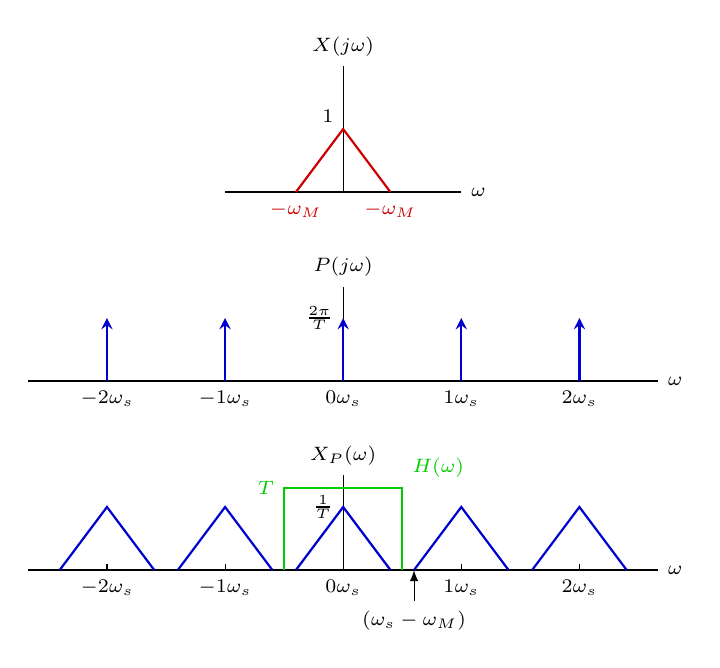
\begin{tikzpicture}[xscale=0.5, yscale=0.8]
    	\def\wm{1.2}
    	\def\ws{3.0}    	
        \draw (0,0) ++(-3,0) -- ++(6,0) node[anchor=west] {\scriptsize $\omega$};
        \draw (0,0) -- ++(0,2) node[anchor=south] {\scriptsize$X(j\omega)$};
        \draw[red!80!black, thick] (0,0) ++(-\wm,0) node[anchor=north] {\scriptsize$-\omega_M$} -- ++(\wm,1) -- +(\wm, -1) node[anchor=north] {\scriptsize$-\omega_M$};
        \node at (0, \wm) [anchor=east] {\scriptsize $1$};

        \begin{scope}[yshift=-3cm]
	        \draw (0,0) ++(-8,0) -- ++(16,0) node[anchor=west] {\scriptsize $\omega$};
	        \draw (0,0) -- ++(0,1.5) node[anchor=south] {\scriptsize$P(j\omega)$};
	        \foreach \w in {-2, -1, 0, 1, 2}
	        {
	            \draw[blue!80!black, thick, -stealth] (\w*\ws, 0) node[anchor=north, color=black] {\scriptsize $\w\omega_s$} -- ++(0, 1);
	        }
        	\node at (0, 1) [anchor=east] {\scriptsize $\frac{2\pi}{T}$};	
	\end{scope}
\pause
	
        \begin{scope}[yshift=-6cm]
	        \draw (0,0) ++(-8,0) -- ++(16,0) node[anchor=west] {\scriptsize $\omega$};
	        \draw (0,0) -- ++(0,1.5) node[anchor=south] {\scriptsize$X_P(\omega)$};
	        \foreach \w in {-2, -1, 0, 1, 2}
	        {
	
	            \draw[blue!80!black, thick] (\w*\ws, 0) ++(-\wm, 0) -- ++(\wm, 1) -- ++(\wm, -1);
	            \node at  (\w*\ws, 0) [anchor=north, color=black] {\scriptsize $\w\omega_s$};
	            \draw (\w*\ws, 0)  -- ++(0, 0.1);
	        }
	        \node at (0, 1) [anchor=east] {\scriptsize $\frac{1}{T}$};	
	        \draw[latex-] (\ws - \wm, 0) -- ++(0,-0.5) node  [anchor=north] {\scriptsize $(\omega_s - \omega_M)$};		
	\pause
 	\draw[thick, green!80!black] (-\ws/2, 0) -- ++(0,1.3) node [anchor=east] {\scriptsize $T$} -- ++(\ws, 0) node [anchor=south west] {\scriptsize $H(\omega)$} -- ++(0, -1.3);

	\end{scope}	

    \end{tikzpicture} 